\documentclass[pdf,notheorems,10pt,intlimits,unicode]{beamer}
\usetheme[numbers,totalnumbers,compress,nologo]{Statmod}
\usefonttheme[onlymath]{serif}
\setbeamertemplate{navigation symbols}{}

\usepackage[utf8]{inputenc}
\usepackage[T2A]{fontenc}
\usepackage[russian]{babel}

\usepackage{graphicx,subcaption,ragged2e}
\usepackage{caption}
\usepackage{slashbox}

\usepackage{tikz}
% \usepackage{ragged2e}
\usepackage{hhline}
\usepackage{array}
\usepackage[table,x11names]{xcolor}

\usepackage{amsthm}
\usepackage{amsmath}
\usepackage{amssymb}
\usepackage{mathtools}
\usepackage{hhline}
\usepackage{xcolor}
\usepackage{array}
\usepackage{bbm}
\usepackage{bm}

\AtBeginSection[]{
  \begin{frame}[noframenumbering]
  \vfill
  \centering
  \begin{beamercolorbox}[sep=8pt,center,shadow=true,rounded=true]{title}
    \usebeamerfont{title}\insertsectionhead\par%
  \end{beamercolorbox}
  \vfill
  \end{frame}
}

\setbeamerfont{institute}{size=\normalsize}
\setbeamercolor{bluetext_color}{fg=blue}

\newtheorem{remark}{Замечание}
\newtheorem{algorithm}{Алгоритм}
\newtheorem{assumption}{Предположение}
\newtheorem{definition}{Определение}

\newcommand{\bfxi}{\boldsymbol{\xi}}
\newcommand{\bluetext}[1]{{\usebeamercolor[fg]{bluetext_color}#1}}
\newcommand{\redtext}[1]{{\usebeamercolor[fg]{redtext_color}#1}}

\setcounter{tocdepth}{2}

\title[Метод Монте-Карло SSA]{Алгоритмы извлечения сигнала из временных рядов с использованием метода Monte Carlo SSA
 }

\author{Потешкин Егор Павлович, гр.24.М22-мм}

\institute[Санкт-Петербургский Государственный Университет]{%
	\small
	Санкт-Петербургский государственный университет\\
	Математическое моделирование, программирование и искусственный интеллект\\
	Кафедра статистического моделирования \vspace{1.25cm}

  % Научный руководитель --- д.\,ф.-м.\,н. Н.\,Э.~Голяндина\\
  % Рецензент --- программист A.\,Ю.~Шлемов, Майкрософт
}

\date{Санкт-Петербург, 2026}

\input{../letters_series_mathbb.tex}

% \graphicspath{../img/}

\begin{document}

\begin{frame}[plain]
    \titlepage
    \note{Научный руководитель  д.ф.-м.н., доцент Голяндина\,Н.\,Э.,\\
        кафедра статистического моделирования}
\end{frame}

% \begin{frame}{Обзор}

%     \begin{enumerate}
%         \item Мотивация и постановка задачи.
%         \item Сравнение методов оценки параметров шума.
%         \item Описание метода SSA и критерия MC-SSA.
%         \item Численное сравнение выбора проекционных векторов в MC-SSA: собственные векторы vs. косинусы.
%         \item Описание существующих методов автоматической идентификации сигнала.
%         \item Описание разработанного метода autoMCSSA и подхода к выбору его параметров.
%         \item Описание разработанного метода SSA-AidMC и численное сравнение методов.
%         \item Выводы и дальнейшие планы.
%     \end{enumerate}

% \end{frame}

% \begin{frame}{Мотивация и актуальность}

%     Временной ряд $\tX=(x_1,\ldots,x_N)$~--- последовательность наблюдений, упорядоченных по времени.\medskip

%     \bluetext{Примеры}: Объемы продаж по месяцам, замеры температуры в течении нескольких лет.\medskip

%     Цель анализа временных рядов~--- определение его структуры, выявление закономерностей и трендов, а также прогнозирование будущих значений.\medskip

%     \bluetext{Приложение}: медицина, финансы, климатология и др.

% \end{frame}

\begin{frame}{Введение}

    $\tX=(x_1,\ldots,x_N)$~--- временной ряд длины $N$.\medskip

    \bluetext{Модель}: $\tX=\tT+\tP+\tR$, где $\tT$~--- тренд, $\tP$~--- периодическая компонента и $\tR$~--- шум, случайная составляющая.\medskip

    \bluetext{Проблема}: Как автоматически выделить сигнал $\tS=\tT+\tP$?\medskip
    % \begin{enumerate}
    %     \item Как выделить неслучайные компоненты $\tT$ и $\tH$?
    %     \item Как проверить наличие сигнала $\tS=\tT+\tH$?
    % \end{enumerate}

    \bluetext{Методы}:
    \begin{enumerate}
        \item Singular spectrum analysis (SSA)~[Broomhead and King, 1986], [Golyandina, Nekrutkin and Zhigljavsky, 2001] для выделения сигнала $\tS$.
        \item Monte Carlo SSA (MC-SSA)~[Allen and Smith, 1996] для проверки гипотезы $H_0:\tS=0$.
    \end{enumerate}\medskip

    \textcolor{red}{Но}: один из шагов SSA требует визуального анализа для определения сигнальных компонент, необходима автоматизация этого шага.

\end{frame}

\begin{frame}{Введение. Продолжение}

    Существует метод автоматического выделения тренда и периодик~[Golyandina, Dudnik and Shlemov, 2025].\smallskip

    \textcolor{red}{Недостаток}: метод работает только если компоненты доминируют над шумом.\smallskip

    \bluetext{Основная цель работы}: разработать метод автоматического выделения сигнала, который не обязательно доминирует над шумом.\smallskip

    Данный метод будет основан на методе MC-SSA для обнаружения сигнала и SSA его выделения, поэтому работа выстроена следующим образом:
    \begin{enumerate}
        \item Описание методов SSA и MC-SSA.
        \item Исследование выбора проекционных векторов в методе MC-SSA.
        \item Применение метода MC-SSA на практике.
        \item Описание существующего метода автоматической идентификации.
        \item Описание разработанного метода автоматической идентификации и его численное сравнение с существующим методом.
    \end{enumerate}
    % \bluetext{Рассматриваемые в работе проблемы}:
    % \begin{enumerate}
    %     \item Для критерия MC-SSA обычно используется модель красного шума (AR(1)), но в геофизике, гидрологии и финансах ряды часто обладают длинной памятью.
    %     \item Параметры шума на практике неизвестны и выбор метода для их оценки сильно влияет на качество их оценки и тем самым на результат критерия.
    %     \item Самый популярный вариант MC-SSA является радикальным критерием и чтобы сделать его точным, нужно провести очень трудоемкую процедуру.
    % \end{enumerate}

\end{frame}

% \section{Глава 1. Процессы с длинной памятью и оценка параметров шума}

% \begin{frame}{Введение}

%     \begin{itemize}
%         \item Для критерия MC-SSA обычно используется модель красного шума (AR(1)), которая широко используется в финансах и климатологии.\smallskip
%         \item Однако, такая модель плохо описывает временные ряды, обладающие длинной памятью, то есть ряды, автокорреляционная функция которых убывает медленнее, чем экспоненциальное затухание.\smallskip
%         \item Процессы с длинной памятью довольно распространены в реальном мире, поэтому при анализе таких рядов с помощью MC-SSA нужно учитывать и эту модель.
%     \end{itemize}
    
% \end{frame}

% \begin{frame}{Обозначения и известные результаты: процессы с длинной памятью}

%     \begin{definition}
%         Говорят, что стационарный процесс $\bm\xi$ обладает длинной памятью, если
%         \[
%             \sum_{h=0}^H|\gamma(h)| \rightarrow \infty,
%         \]
%         при $H\to\infty$. Иначе говорят, что $\bm\xi$ обладает короткой памятью.
%     \end{definition}\medskip

%     Пример процесса с короткой памятью: процесс $\text{ARMA}(p, q)$.\medskip

%     Пример процесса с длинной памятью: процесс $\text{ARFIMA}(p, d, q)$:
%     \[
%         Y_t=(1-L)^{-d}X_t, \quad d < 1 / 2,
%     \]
%     где $X_t$~--- модель $\text{ARMA}(p, q)$.

% \end{frame}

% \begin{frame}{Численное исследование: оценка параметров шума}

%     \bluetext{Модель}: $\tX=\bm\xi$, где $\bm\xi$~--- модель AR$(1)$, ARFIMA$(0, d, 0)$ или ARFIMA$(1, d, 0)$.\medskip

%     \bluetext{Задача}: сравнить точность различных методов оценки параметров шума $\bm\xi$ для разных длин ряда $N$.\medskip

%     \bluetext{Методы}: MLE (с известным средним $\mu$ и его оценкой $\hat\mu=\bar x$), аппроксимация MLE (H\&R) и метод Уиттла (Whittle).\medskip

%     \bluetext{Результат}: численные эксперименты показали, что для реальных рядов с неизвестным средним метод Уиттла дает наименее смещенную оценку и обладает наименьшей вычислительной сложностью $O(N\log N)$ благодаря использованию FFT периодограммы.

% \end{frame}

\section{Глава 1. Метод MC-SSA}

\begin{frame}{Обозначения и известные результаты: Метод SSA}

    \bluetext{Входные данные}: временной ряд $\tX=(x_1,\ldots,x_N)$.\medskip

    \bluetext{Параметр}: длина окна $L$, $1<L<N$.\medskip

    \bluetext{Результат}: $m$ восстановленных составляющих временного ряда.\medskip
    \begin{enumerate}
        \item \textbf{Вложение}: $\bfX=\cT(\tX)=[X_1:\ldots:X_K]$, где $X_i=(x_1,\ldots,x_{i+L-1})^\rmT$, $K=N-L+1$.\smallskip
        \item \textbf{Разложение}: $\bfX=\sum_{i=1}^r \sigma_i P_i Q_i^\rmT=\bfX_1+\ldots+\bfX_r$, $\operatorname{rank}\bfX_i=1$.\smallskip
        \item \textbf{Группировка}: $\bfX=\bfX_{I_1}+\ldots+\bfX_{I_m}$, где $\bfX_{I_k}=\sum_{i\in I_k}\bfX_i$.\smallskip
        \item \textbf{Восстановление}: $\tX=\widetilde\tX_{I_1}+\ldots+\widetilde\tX_{I_m}$, где $\widetilde\tX_{I_k}=\cT^{-1}\circ\cH(\bfX_{I_k})$.
    \end{enumerate}

\end{frame}

\begin{frame}{Обозначения и известные результаты: Toeplitz SSA}
	Модификации SSA отличаются только шагом разложения.\medskip

	Basic SSA: сингулярное разложение траекторной матрицы, универсальный метод.\medskip

	Toeplitz SSA: теплицево разложение траекторной матрицы, имеет преимущество для стационарных рядов:
	\begin{equation*}
		\bfX=\sum_{i=1}^L\sigma_i P_iQ_i^\rmT = \bfX_1+\ldots +\bfX_L,
	\end{equation*}
	где $Q_i=\bfX^\rmT P_i/\sigma_i$, $\sigma_i=\|\bfX^\rmT P_i\|$, $\{P_i\}_{i=1}^L$ "--- собственные векторы матрицы $\bfT$ с элементами
	\begin{equation*}
		t_{ij} = \frac{1}{N - |i - j|}\sum_{m=1}^{N-|i-j|}x_mx_{m+|i-j|},1\leqslant i,j\leqslant L.
	\end{equation*}

\end{frame}

\begin{frame}{Обозначения и известные результаты: Multiple Monte Carlo SSA~[Golyandina, 2023]}

    \bluetext{Модель}: $\tX=\tS + \bm\xi$, где $\tS$ "--- сигнал (колебания с какой-то частотой), $\bm\xi$ "--- стационарный процесс с нулевым средним.\medskip

    \bluetext{Задача}: проверить $H_0:\tS=0$ "--- отсутствие сигнала.\medskip

    \bluetext{Метод}: Multiple Monte Carlo SSA~[Golyandina, 2023] (далее просто MC-SSA).\medskip

    \bluetext{Входные данные}: временной ряд $\tX$.

    \bluetext{Параметры}: длина окна $L$, выбор векторов $W_1,\ldots,W_H\in \mathbb{R}^{L}$, модель шума $\bm\xi$, количество суррогатных реализаций $G$.
    \begin{enumerate}
        \item Строятся статистики критерия $\widehat p_k=\|\bfX^\rmT W_k\|^2$, $k=1,\ldots,H$.
        \item Оцениваются их распределения на основе $G$ суррогатных реализаций $\bm\xi$.
        \item Строятся предсказательные интервалы с поправкой на множественные сравнения с уровнем доверия $(1-\alpha)$.
    \end{enumerate}

    % Далее предполагаем, что $\boldsymbol{\xi}$ "--- красный шум, причем с известными параметрами.

\end{frame}

\begin{frame}{Обозначения и известные результаты: поправка неточных критериев}

    Приведем алгоритм, преобразовывающий неточный критерий (консервативный или радикальный) в асимптотически точный.\medskip

    Зафиксируем $H_0$, уровень значимости $\alpha^*$, количество выборок $M$ для оценки $\alpha_I(\alpha)$ и их объем $N$:
    \begin{enumerate}
        \item Моделируется $M$ выборок объема $N$ при верной $H_0$.
        \item По моделированным данным строится зависимость ошибки первого рода от уровня значимости $\alpha_I(\alpha)$.
        \item Рассчитывается формальный уровень значимости: $\widetilde{\alpha}^*=\alpha_I^{-1}(\alpha^*)$. Критерий с таким уровнем значимости является асимптотически точным при $M\to\infty$.
    \end{enumerate}

\end{frame}

\begin{frame}{Обозначения и известные результаты: выбор векторов для проекции в методе MC-SSA}
    Одним из параметров MC-SSA является выбор векторов $W_k$, на которые будет производится проекция столбцов матрицы $\bfX$.\medskip

    Наиболее распространенный вариант MC-SSA использует векторы $W_k$, являющимися собственными векторами матрицы $\bfX\bfX^\rmT$ или $\bfT$ (далее будем называть его критерием <<ev>>).\medskip
    
    \bluetext{Плюс}: если $H_0$ отверглась, можно восстановить сигнал с помощью SSA на основе значимых $W_k$.\medskip
    
    \textcolor{red}{Минус}: этот вариант дает радикальный критерий и преобразование его в точный~--- очень трудоемкая задача.



    % В данной работе рассмотрены два варианта выбора $W_k$:
    % \begin{enumerate}
    %     \item Собственные векторы матрицы $\bfX\bfX^\rmT$ или $\bfT$.
    %     \item Косинусы с равноотстоящими частотами $\omega_k=k/(2L)$:
    %           \[
    %               V_k=
    %               \begin{pmatrix}
    %                   \cos(2\pi\omega_k 1) \\
    %                   \ldots               \\
    %                   \cos(2\pi\omega_k L)
    %               \end{pmatrix},\quad W_k=\frac{V_k}{\|V_k\|},\quad k=1,\ldots,L.
    %           \]
    % \end{enumerate}\medskip

    % Далее будем называть критерий MC-SSA с таким выбором векторов $W_k$ <<ev>> и <<cos>> соответственно.

\end{frame}

\begin{frame}{Обозначения и известные результаты: выбор векторов для проекции в методе MC-SSA}

    Можно использовать косинусы в качестве векторов для проекции (далее критерий <<cos>>):
    \[
        V_k=
        \begin{pmatrix}
            \cos(2\pi\omega_k 1) \\
            \ldots               \\
            \cos(2\pi\omega_k L)
        \end{pmatrix},\quad W_k=\frac{V_k}{\|V_k\|},\quad k=1,\ldots,L,
    \]
    где $\omega_k=k/(2L)$.\medskip

    \bluetext{Мотивация}: собственные векторы стационарного процесса представляют собой гармоники с равноотстоящими частотами.\medskip

    \bluetext{Плюс}: такой критерий является точным.\medskip

    \bluetext{Задача}: сравнить критерий <<cos>> с критерием <<ev>> по мощности.

\end{frame}

\begin{frame}{Численное сравнение критериев MC-SSA}

    \bluetext{Модель}: $\tX=\tS+\bm\xi$, где
    \begin{enumerate}
        \item $\tS=\{Ae^{\alpha n}\cos(2\pi n\omega)\}_{n=1}^N$~--- экспоненциально-модулированная гармоника.
        \item $\bm\xi$~--- стационарный процесс с известными параметрами.
    \end{enumerate}\medskip

    \bluetext{Задача}: сравнить ошибку первого рода и мощность критериев при различных вариантах сигнала $\tS$:
    \begin{enumerate}
        \item $a=0$, $L\omega$~--- целые;
        \item $a=0$, $L\omega$~--- нецелые;
        \item $a\ne0$, $L\omega$~--- целые;
        \item $a=0$, $L\omega$~--- нецелые.
    \end{enumerate}

\end{frame}

\begin{frame}{Численное сравнение критериев MC-SSA: ошибка первого рода}

    % \begin{figure}
    %     \centering
    %     \subfloat[Собственные векторы $\bfT$]{\label{a}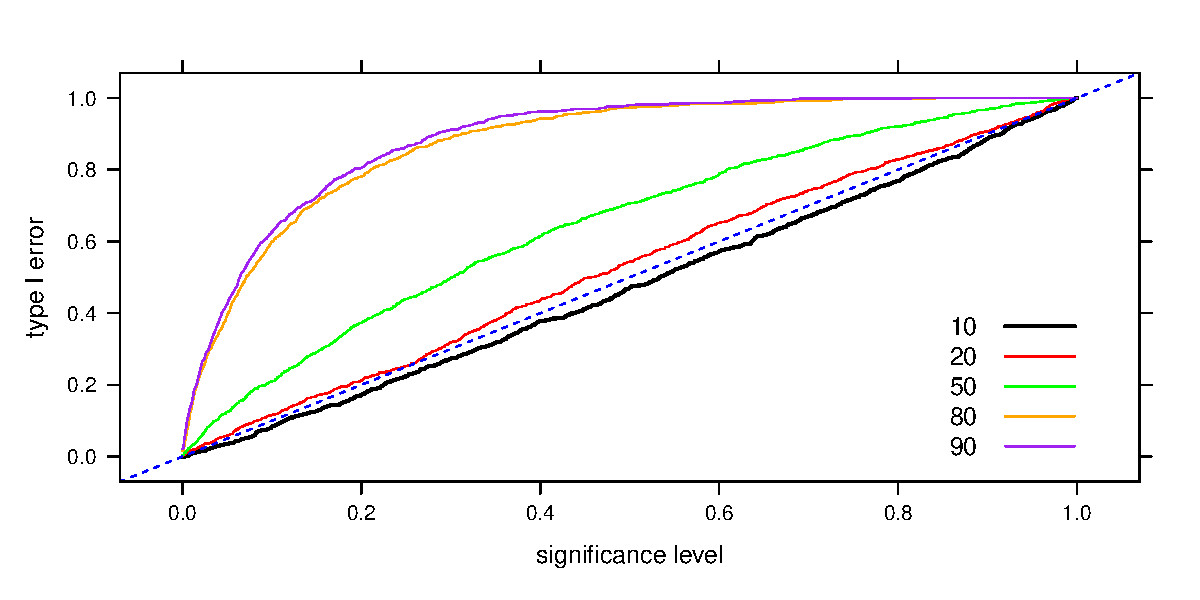
\includegraphics[width=.5\linewidth]{../img/mcssa_comp_alphaI_ev.pdf}}\hfill
    %     \subfloat[Собственные векторы $\bfX\bfX^\rmT$]{\label{b}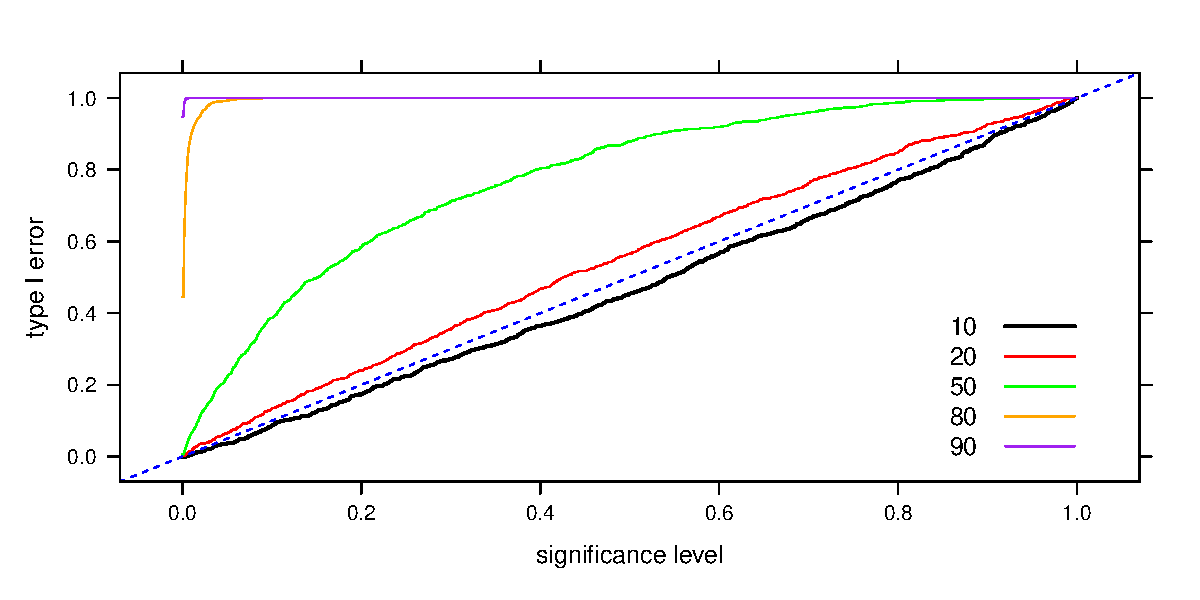
\includegraphics[width=.5\linewidth]{../img/mcssa_comp_alphaI_ev_svd.pdf}}\par
    %     \subfloat[Косинусы]{\label{c}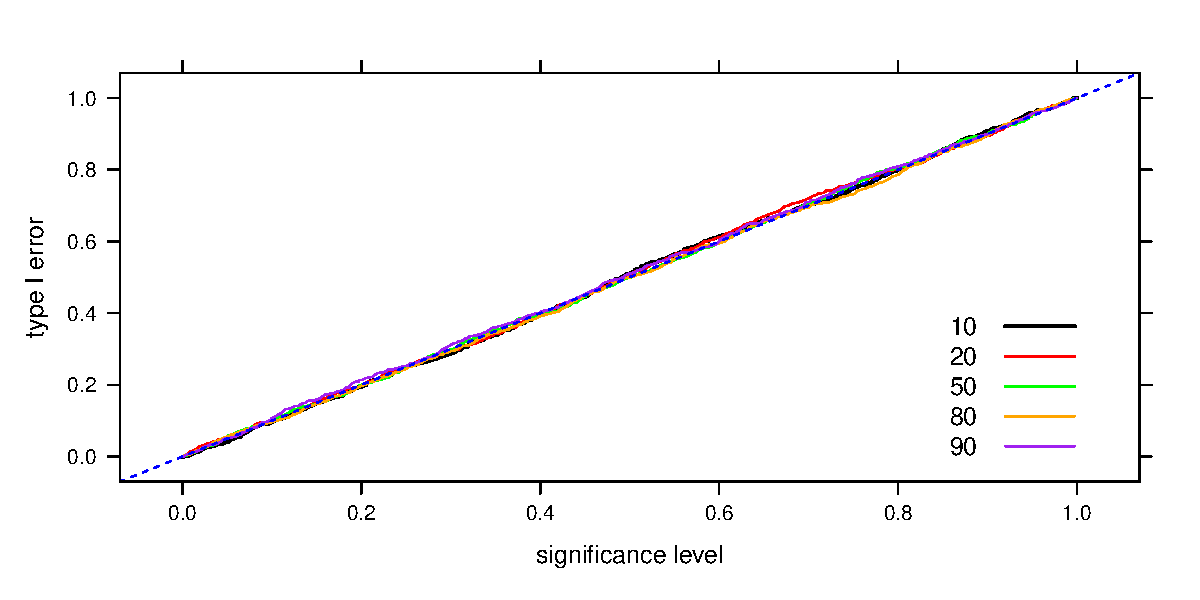
\includegraphics[width=.5\linewidth]{../img/mcssa_comp_alphaI_cos.pdf}}
    %     \caption{Ошибка первого рода}
    %     \label{fig:mcssa_comp_alphaI}
    % \end{figure}
    \begin{table}[h!]
        \centering
        \caption{Ошибка первого рода при уровне значимости $\alpha^*=0.1$}
        \scalebox{0.8}{
            \begin{tabular}{c|c|c|c|c|c}
                                                    & $L=10$ & $L=20$ & $L=50$ & $L=80$ & $L=90$ \\
                \hline
                Собственные векторы $\bfX\bfX^\rmT$ & 0.087  & 0.133  & 0.387  & 1      & 1      \\
                \hline
                Собственные векторы $\bfT$          & 0.083  & 0.116  & 0.21   & 0.599  & 0.626  \\
                \hline
                Косинусы                            & 0.097  & 0.101  & 0.103  & 0.096  & 0.107  \\
            \end{tabular}
        }
    \end{table}\medskip

    \bluetext{Вывод}: для векторов $W_k$, порожденных исходным рядов, критерий MC-SSA радикален для $L>10$, для косинусов критерий точен для любой длины окна.

\end{frame}

\begin{frame}{Численное сравнение критериев MC-SSA: мощность}

    \begin{table}[h!]
        \centering
        \caption{Мощность поправленных критериев при уровне значимости $\alpha^*=0.1$}
        \scalebox{0.65}{
            \begin{tabular}{c|c|c|c|c|c}
                $a=0$, $L\omega$~--- целые                      & $L=10$ & $L=20$ & $L=50$ & $L=80$ & $L=90$ \\
                \hline
                Проекция на собственные векторы $\bfT$          & 0.424  & 0.484  & 0.525  & 0.582  & 0.646  \\
                \hline
                Проекция на косинусы                            & 0.543  & 0.546  & 0.546  & 0.614  & 0.646  \\
                \hhline{======}
                $a=0$, $L\omega$~--- нецелые                    & $L=10$ & $L=20$ & $L=50$ & $L=80$ & $L=90$ \\
                \hline
                Проекция на собственные векторы $\bfT$          & 0.349  & 0.432  & 0.425  & 0.497  & 0.537  \\
                \hline
                Проекция на косинусы                            & 0.475  & 0.431  & 0.403  & 0.505  & 0.488  \\
                \hhline{======}
                $a\ne0$, $L\omega$~--- целые                    & $L=10$ & $L=20$ & $L=50$ & $L=80$ & $L=90$ \\
                \hline
                Проекция на собственные векторы $\bfX\bfX^\rmT$ & 0.329  & 0.303  & 0.307  & --     & --     \\
                \hline
                Проекция на косинусы                            & 0.480  & 0.347  & 0.163  & 0.228  & 0.299  \\
                \hhline{======}
                $a\ne0$, $L\omega$~--- нецелые                  & $L=10$ & $L=20$ & $L=50$ & $L=80$ & $L=90$ \\
                \hline
                Проекция на собственные векторы $\bfX\bfX^\rmT$ & 0.298  & 0.306  & 0.282  & --     & --     \\
                \hline
                Проекция на косинусы                            & 0.469  & 0.302  & 0.157  & 0.209  & 0.249  \\
            \end{tabular}
        }
    \end{table}

    \bluetext{Вывод}: критерий <<cos>> является более предпочтительным, поскольку является точным и по мощности не уступает, а в некоторых случаях даже превосходит критерий <<ev>>.

\end{frame}

\begin{frame}{Применение MC-SSA к реальным временным рядам}

    \begin{itemize}
        \item До этого предполагалось, что параметры шума $\bm\xi$ известны.\medskip
        \item В реальности они неизвестны и их нужно оценивать. Тогда перед алгоритмом MC-SSA необходимо оценить параметры модели $\bm\xi$ по исходному ряду.\medskip
        \item Также для критерия MC-SSA обычно используется модель красного шума (AR(1)), однако в геофизике, гидрологии и финансах ряды часто обладают длинной памятью.\medskip
        \item Неправильно выбранная модель делает критерий радикальным либо консервативным. Первое влечет за собой неприменимость критерия, а второе~--- уменьшение мощности критерия.\medskip
        % \item В работе~[Потешкин, 2024] показано, что оценка параметров несильно искажает критерий.\medskip
        % \item При оцененной модели шума $\bm\xi$ критерий <<cos>> становится консервативным, а критерий <<ev>>~--- менее радикальным.
        \item На данный момент в работе преимущественно используется модель красного шума, однако в дальнейшем планируется добавить больше исследований рядов с длинной памятью.
    \end{itemize}

\end{frame}

\begin{frame}{Обозначения и известные результаты: процессы с длинной памятью}

    \begin{definition}
        Говорят, что стационарный процесс $\bm\xi$ обладает \textbf{длинной} памятью, если
        \[
            \sum_{h=0}^H|\gamma(h)| \rightarrow \infty,
        \]
        при $H\to\infty$. Иначе говорят, что $\bm\xi$ обладает \textbf{короткой} памятью.
    \end{definition}\medskip

    Пример процесса с короткой памятью: процесс $\text{ARMA}(p, q)$.\medskip

    Пример процесса с длинной памятью: процесс $\text{ARFIMA}(p, d, q)$:
    \[
        Y_t=(1-L)^{-d}X_t, \quad d < 1 / 2,
    \]
    где $X_t$~--- модель $\text{ARMA}(p, q)$.

\end{frame}

\begin{frame}{Численное исследование: оценка параметров шума}

    \bluetext{Модель}: $\tX=\bm\xi$, где $\bm\xi$~--- модель AR$(1)$, ARFIMA$(0, d, 0)$ или ARFIMA$(1, d, 0)$.\medskip

    \bluetext{Задача}: сравнить точность различных методов оценки параметров шума $\bm\xi$ для разных длин ряда $N$.\medskip

    \bluetext{Методы}: MLE (с известным средним $\mu$ и его оценкой $\hat\mu=\bar x$), аппроксимация MLE~[Haslett and Raftery, 1989] и метод Уиттла~[Whittle, 1953].\medskip

    \bluetext{Результат}: численные эксперименты показали, что для реальных рядов с неизвестным средним метод Уиттла дает наименее смещенную оценку и обладает наименьшей вычислительной сложностью $O(N\log N)$ благодаря использованию FFT периодограммы.

\end{frame}

\begin{frame}{Модификация MC-SSA по части спектра}

    \begin{itemize}
        \item Можно убрать неинтересующую нас часть спектра, задав диапазоны нерассматриваемых частот $\mathcal{B}=\bigcup_j[\omega_{j_1}, \omega_{j_2}]$.\smallskip
        \item Таким образом, в алгоритме MC-SSA из рассмотрения уйдут все векторы $W_k$, частота $\omega_k$ которых попадает в $\mathcal{B}$.\smallskip
        \item Оценка параметров по части спектра возможна с помощью правдоподобия Уиттла по части спектра (еще один плюс этого метода):
              \begin{equation*}
                  \ell_{W_\text{part}}(\bm\varphi; \mathcal{B})=-\frac{1}{|J_{\mathcal{B}^\complement}|}\sum_{j\in J_{\mathcal{B}^\complement}}\left(\ln f_{\bm\xi}(\omega_j; \bm\varphi) + \frac{I(\omega_j)}{f_{\bm\xi}(\omega_j; \bm\varphi)}\right),
              \end{equation*}
              где $\bm\varphi$~--- вектор параметров шума $\bm\xi$, $f_{\bm\xi}$~--- спектральная плотность шума $\bm\xi$, $I$~--- периодограмма исходного ряда, $J_{\mathcal{B}^\complement}=\{j \in \{1,\ldots, m\}:~\omega_j=j/N \not\in \mathcal{B}\}$, $m=\lfloor (N-1)/2 \rfloor$.\smallskip
        \item Далее под MC-SSA будет подразумеваться именно эта модификация.

    \end{itemize}

\end{frame}

\section{Глава 2. Методы автоматической идентификации компонент}

\begin{frame}{Введение}

    \begin{itemize}
        \item После применения MC-SSA, если $H_0:\tS=0$ отверглась, необходимо выделить значимый сигнал.\medskip
        \item Критерий MC-SSA с косинусами в качестве векторов для проекции не позволяет выделить сигнал.\medskip
        \item Однако, критерий дает информацию о значимых частотах, которую можно использовать. 
    \end{itemize}

\end{frame}

\begin{frame}{Обозначения и известные результаты: Автоматическая группировка в SSA}

    Для ряда $\tX$ длины $N$ и $0\leqslant\omega_1\leqslant\omega_2\leqslant0.5$ определим меру~[Алесандров, Голяндина, 2004]
    $$
        T(\tX; \omega_1,\omega_2)=\frac{1}{\|\tX\|^2}\sum_{k:\omega_1\leqslant k / N \leqslant \omega_2}\Pi(k / N),
    $$
    где $\Pi$~--- односторонняя периодограмма ряда $\tX$:
    \begin{equation*}
        \Pi(k / N)=
        \begin{cases}
            I(k / N) + I(1 - k / N), & \text{для } 0<k<N/2, \\
            I(k / N),                & \text{иначе}.
        \end{cases}
    \end{equation*}
    Величину $T(\tX; \omega_1, \omega_2)$ можно рассматривать как долю вклада частот, содержащегося в интервале $[\omega_1, \omega_2]$.

\end{frame}

\begin{frame}{Обозначения и известные результаты: Автоматическая идентификация тренда~[Александров, Голяндина, 2004]}

    \begin{algorithm}[Автоматическая идентификация тренда]
        \bluetext{Входные данные}: элементарные восстановленные компоненты $\tX^{(j)}$, $j\in J$, порог низких частот $\omega_0$, порог вклада низких частот $T_\text{low}\in[0, 1]$.\medskip

        \bluetext{Результат}: компоненты, относящиеся к тренду, оценка тренда.\medskip

        \begin{enumerate}
            \item Вычислить $T_j=T(\tX^{(j)};0,\omega_0)$ для каждого $j\in J$.\smallskip
            \item Определить компоненты $J_\text{Trend}=\{j\in J:~T_j > T_\text{low}\}$, относящиеся к тренду, вычислить оценку тренда $\hat \tT=\sum\limits_{j\in J_\text{Trend}} \tX^{(j)}$.
        \end{enumerate}
    \end{algorithm}

    \bluetext{Алгоритм autoEOSSA}~[Golyandina, Dudnik, Shlemov, 2023]: применение переразложения EOSSA к первым $r$ компонентам и последующее применение алгоритма автоматической идентификации тренда.
\end{frame}

\begin{frame}{Автоматическая идентификация периодики: алгоритм}

    \begin{algorithm}[Автоматическая идентификация периодики]
        \bluetext{Входные данные}: Ряды $\tX^{(j)}$, $j\in J$, частота $\omega\in(0, 0.5]$, радиус $\delta \geqslant 0$, порог $T_0\in[0, 1]$, количество компонент $d$.\medskip

        \bluetext{Результат}: Индексы рядов, относящихся к периодике с частотой $\omega$, оценка $\hat\tP$.\medskip

        \begin{enumerate}
            \item Вычислить $T_j=T(\tX^{(j)};\omega - \delta,\omega + \delta)$ для каждого $j\in J$.\smallskip
            \item Из множества $J_\text{signif}=\{j\in J:~T_j > T_0\}$ выбрать $\min(d, |J_\text{signif}|)$ элементов, соответствующих рядам с наибольшим $\mathsf{MSS}\left(\tX^{(j)}\right)=\frac{1}{N}\sum^{N}_{i=1}\left(x^{(j)}_i\right)^2$. Обозначим множество этих индексов за $J_\text{Periodic}$.\smallskip
            \item Вычислить оценку периодики $\hat \tP=\sum\limits_{j\in J_\text{Periodic}} \tX^{(j)}$.
        \end{enumerate}
    \end{algorithm}

\end{frame}

\begin{frame}{Автоматическая идентификация периодики: замечания}

    \begin{itemize}
        \item   В алгоритме ряды $\tX^{(j)}$ не обязательно являются элементарно восстановленными компонентами. Это могут быть уже сгруппированные (например, с помощью метода регулярности углов~[Жорникова, 2018]) ряды: в таком случае $d=1$.
        \item  Если $\tX^{(j)}$~--- элементарные восстановленные компоненты, то, учитывая, что экспоненциально-моделированная гармоника описывается одной или двумя компонентами, в качестве параметра $d$ логично взять
              \begin{equation}\label{eq:d_cos}
                  d_{\cos}(\omega)=
                  \begin{cases}
                      2, & \text{для } \omega\in(0, 0.5), \\
                      1, & \text{иначе}.
                  \end{cases}
              \end{equation}
        \item Для применения метода необходимо знать сигнальную частоту $\omega$: ее можно получить с помощью метода MC-SSA.
    \end{itemize}

\end{frame}

% \begin{frame}{Алгоритм автоматической идентификации трендовых и периодических компонент~[Дудник, 2025]}

%     \begin{algorithm}[Алгоритм автоматической идентификации трендовых и периодических компонент]
%         Входные данные: временной ряд $\tX$, длина окна $L_\text{SSA}$, оценка ранга сигнала $r$, порог $t_0$, порог $p_0$, порог низких частот $\omega_0$, порог вклада низких частот $T_{\text{low}}$.\medskip

%         Результат: Множества индексов, соответствующие тренду и периодикам.\medskip

%         \begin{enumerate}
%             \item Применить к исходному ряду алгоритм autoEOSSA($r, \omega_0, T_{\text{low}}$). Результат: множество индексов $J_\text{Trend}$, которое соответствует тренду.\smallskip
%             \item Применить к компонентам с индексами из множества $J\setminus J_\text{Trend}$ модифицированный метод регулярности углов. Результат: множество индексов $J_\text{Periodics}$, которое соответствует периодикам.
%         \end{enumerate}
%     \end{algorithm}

% \end{frame}

\begin{frame}{Обозначения и известные результаты: Метод регулярности углов~[Жорникова, 2018]}

    \begin{itemize}
        \item \bluetext{Что делает метод?} Метод идентифицирует э-м гармоники с частотами $0 < \omega < \frac{1}{2}$.\medskip
        \item \bluetext{Входные данные и параметры}: Левые сингулярные векторы траекторной матрицы. Порог $\tau_0$.\medskip
        \item \bluetext{Идея метода}: Метод использует факт, что углы между последовательными отрезками на двумерной диаграмме сингулярных векторов равны.\medskip
        \item В работе~[Дудник, 2025] метод расширен на случай $\omega=\frac{1}{2}$. \\К параметрам добавился порог $p_0$. Используется регулярность смены знака компоненты.
    \end{itemize}

\end{frame}

\begin{frame}{Обозначения и известные результаты: Метод SSA-Aid~[Дудник, 2025]}

    \begin{figure}[H]
        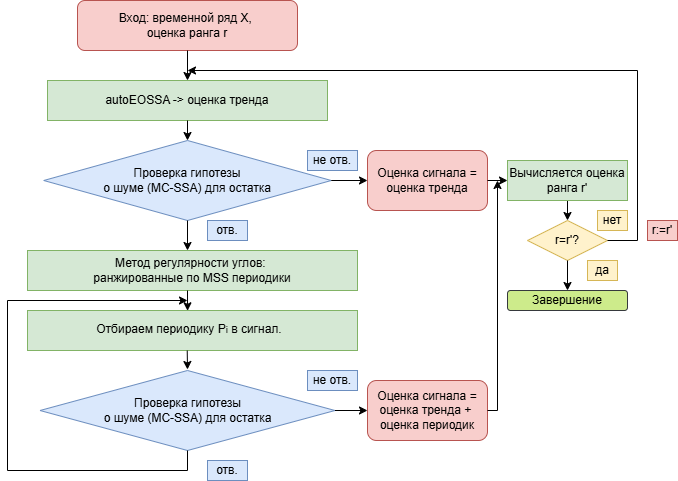
\includegraphics[width=0.8\linewidth]{../img/alg.png}
        \caption{Схема алгоритма SSA-Aid
        }
        \label{fig:wine_decompose_eossa}
    \end{figure}

\end{frame}

% \begin{frame}
%     \begin{algorithm}[Отбор перидики в сигнал ]

%     \end{algorithm}
% \end{frame}

% \begin{frame}
%     \scriptsize
%     \begin{algorithm}[Алгоритм автоматической идентификации компонент, использующий критерий с проверкой гипотезы о белом или красном шуме~\cite{Dudnik2025}]\label{alg:auto_periodic_trend_mc}
% 	Входные данные: временной ряд $\tX$, длина окна $L_\text{SSA}$, длина окна $L_\text{MC-SSA}$, модель шума $\bm\xi$, оценка ранга сигнала $r$, порог $t_0$, порог $p_0$, уровень значимости $\alpha$, порог низких частот $\omega_0$, порог вклада низких частот $T_{\text{low}}$.\\
% 	Выходные данные: разложение оценки сигнала в сумму тренда и периодик $\hat{\tS}=\hat{\tT} + \sum_{k=1}^p\hat{\tP}^{(k)}$, уточненная оценка ранга сигнала $\hat{r}$.
% 	\begin{enumerate}
% 		\item Применить алгоритм autoEOSSA. Результат: множества $J_{\text{Trend}}$ и $J_{\text{Periodics}}$, $\hat \tT\coloneq \sum\limits_{j\in J_\text{Trend}} \tX^{(j)}$.
% 		\item Инициализировать оценку периодик $\hat{\tP}$ нулевым рядом, оценку ранга периодической компоненты $\hat{r}_\text{Periodics} \coloneq 0$ и диапазоны нерассматриваемых частот $\mathcal{B} \coloneq [0, \omega_0]$.
% 		\item Применить алгоритм~\ref{alg:multiple_mc-ssa_part_spectrum} к ряду $\hat{\tS} - \hat{\tT}$. Если нулевая гипотеза не отвергается при уровне значимости $\alpha$, завершить работу алгоритма с $\hat{\tS}=\hat{\tT}$ и $\hat{r}=\hat{r}_\text{Trend}$.
% 		\item Восстановить компоненты, используя множество $J_{\text{Periodics}}$ и ранжируем по величине $\mathsf{MSS}\left(\tX^{(j)}\right)=\frac{1}{N}\sum^{N}_{i=1}\left(x^{(j)}_i\right)^2$ по убыванию. Пусть восстановлено $n_{\mathsf{id}} = |J_{\text{Periodics}}|$ компонент и $\left\{\tX^{(j)}\right\}_{j=1}^{n_{\mathsf{id}}}$~--- полученный набор. Этому набору соответствует множество рангов  $\left\{r_p^{(j)}\right\}_{j=1}^{n_{\mathsf{id}}}$.
% 		\item Для $j = 1, \ldots, n_{\mathsf{id}}$:
% 		\begin{enumerate}\tiny
% 			\item $\hat{\tP} \coloneq \hat{\tP} + \tX^{(j)}$. $\hat{r}_\text{Periodics} \coloneq \hat{r}_\text{Periodic}+r_p^{(j)}$, $\hat{\tN} \coloneq \tX - \hat{\tT} - \hat{\tP}$.
% 			\item Применить к остатку $\hat{\tN}$ алгоритм~\ref{alg:multiple_mc-ssa_part_spectrum}. Если гипотеза не отвергается при уровне значимости $\alpha$, завершить работу алгоритма с $\hat{\tS} =\hat{\tT} + \hat{\tP}$ и $\hat{r}=\hat{r}_\text{Trend}+\hat{r}_\text{Periodics}$.
% 		\end{enumerate}
% 	    \end{enumerate}
%     \end{algorithm}

% \end{frame}

\begin{frame}{Недостатки метода SSA-Aid}

    SSA-Aid, хотя и является довольно мощным методом автоматической идентификации сигнала, обладает двумя критическими недостатками:\medskip
    \begin{enumerate}
        \item Метод использует критерий MC-SSA как хороший критерий проверки гипотезы об отсутствии сигнала в остатке и не использует информацию о значимых частотах, которые дает MC-SSA.\medskip
        \item Если компоненты сигнала не доминируют перед шумом (то есть сначала идут сигнальные компоненты, включая трендовые, потом какое-то количество шумовых, а потом снова сигнальные) метод SSA-Aid не сможет их обнаружить, не захватив с собой шумовые компоненты.
    \end{enumerate}\medskip

    \bluetext{Задача}: разработать метод автоматической идентификации сигнала, который не имеет перечисленных недостатков.

\end{frame}

% \section{Глава 3. Методы автоматической идентификации компонент, использующие критерий MC-SSA для оценки частоты сигнала}

\begin{frame}{Мощность MC-SSA в случае сложного сигнала}
    Модель: $\tX=\tS + \bm\xi$, где $\tS=(s_1,\ldots, s_N)$:
    \[
        s_n=2\cos\left(\frac{2\pi n}{4}\right) + \cos\left(\frac{2\pi n}{8}\right),
    \]
    $N=200$, $\bm\xi$~--- красный шум с $\phi=0.7$, $\sigma^2=1$.

    \begin{figure}[!h]
        \centering
        \begin{subfigure}{0.4\textwidth}
            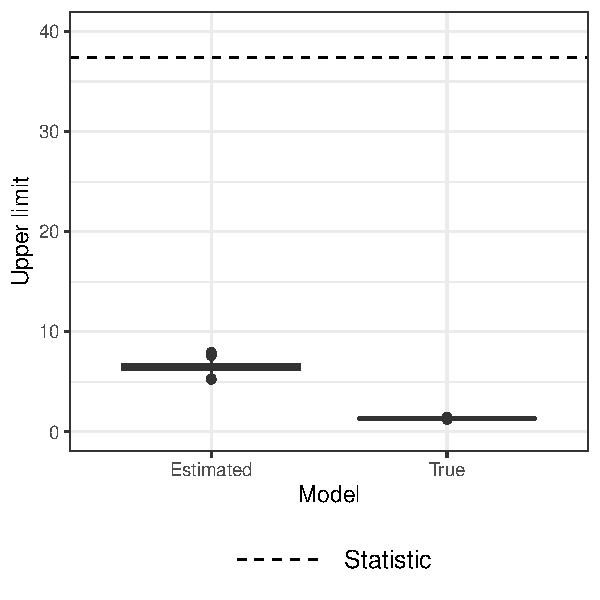
\includegraphics[width=0.92\textwidth]{../img/mcssa_ci_025.pdf}
            \caption{$\omega=0.25$}
            \label{fig:mcssa_ci_1}
        \end{subfigure}
        \begin{subfigure}{0.4\textwidth}
            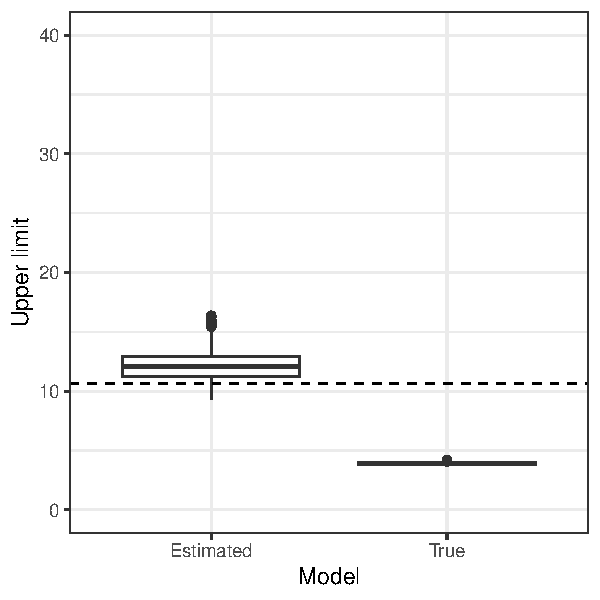
\includegraphics[width=0.92\textwidth]{../img/mcssa_ci_0125.pdf}
            \caption{$\omega=0.125$}
            \label{fig:mcssa_ci_2}
        \end{subfigure}
        \caption{Верхние границы предсказательных интервалов}
        \label{fig:mcssa_ci}
    \end{figure}

\end{frame}

\begin{frame}{Мощность MC-SSA в случае сложного сигнала}
    \begin{itemize}
        \item В случае истинной модели шума обе частоты являются значимыми всегда.\smallskip
        \item Когда параметры шума оцениваются, более сильная часть сигнала ($\omega=0.25$) все еще значима, в то время как более слабая часть ($\omega=0.125$) перестает быть значимой в большинстве случаев.\smallskip
        \item \textcolor{red}{Проблема}: при оцененных параметрах шума критерий MC-SSA может обнаружить не все частоты, принадлежащие сигналу.\smallskip
        \item \bluetext{Решение}: оценивать сигнал последовательно, применяя критерий MC-SSA к остатку до тех пор, пока гипотеза $H_0: \tS=0$ не перестанет отвергаться.
    \end{itemize}
\end{frame}

\begin{frame}{Метод autoMCSSA}
    \footnotesize
    \begin{algorithm}[autoMCSSA]
        \bluetext{Входные данные}: временной ряд $\tX$, элементарные восстановленные компоненты $\tX^{(j)}$, $j\in J$, длина окна $L\in(1, N)$, модель шума $\bm\xi$, уровень значимости $\alpha$, порог низких частот $\omega_0$, радиус $\delta \geqslant 0$, порог $T_0\in[0, 1]$.

        \bluetext{Результат}: индексы периодических компонент $J_\text{Periodics}$, оценка периодик $\hat \tP$.

        \begin{enumerate}\scriptsize
            \item Инициализировать оценку периодик $\hat\tP$ нулевым рядом, множество индексов $J_\text{Periodics} \coloneq \varnothing$ и диапазоны нерассматриваемых частот $\mathcal{B} \coloneq [0, \omega_0]$.
            \item Применить критерий MC-SSA к ряду $\tX$. Если нулевая гипотеза не отвергается при уровне значимости $\alpha$, завершить работу алгоритма.
            \item Если $|J|=0$, завершить работу алгоритма.
            \item Вычислить оценку максимально значимой частоты $\omega^\star$.
            \item Получить компоненты $J_{\omega^\star}$ и оценку периодики $\tP_{\omega^\star}$ с помощью алгоритма автоматической идентификации периодики с рядами $\left\{\tX^{(j)}\right\}_{j\in J}$ и $d=d_{\cos}(\omega^\star)$.
            \item $J_\text{Periodics} \coloneq J_\text{Periodics}\cup J_{\omega^\star}$, $\hat{\tP} \coloneq \hat{\tP} + \tP_{\omega^\star}$, $\hat{\tN} \coloneq \tX - \hat{\tP}$.
            \item Если $|J_{\omega^\star}|=0$, $\mathcal{B} \coloneq \mathcal{B}\cup\left[\omega^\star - \delta, \omega^\star + \delta\right]$.
            \item \label{alg:auto_periodic_trend_modified_3} Применить к остатку $\hat{\tN}$ критерий MC-SSA. Если гипотеза не отвергается при уровне значимости $\alpha$, завершить работу алгоритма.
            \item $J \coloneq J \setminus J_{\omega^\star}$, вернуться к шагу 2.
        \end{enumerate}

    \end{algorithm}

\end{frame}

% \begin{frame}{Метод autoMCSSA}
%     \begin{enumerate}\setcounter{enumi}{3}
%         \item Вычислить оценку максимально значимой частоты $\omega^\star$.\smallskip
%         \item Получить компоненты $J_{\omega^\star}$ и оценку периодики $\tP_{\omega^\star}$ с помощью алгоритма автоматической идентификации периодики с рядами $\left\{\tX^{(j)}\right\}_{j\in J}$ и $d=d_{\cos}(\omega^\star)$~\eqref{eq:d_cos}.\smallskip
%         \item $J_\text{Periodics} \coloneq J_\text{Periodics}\cup J_{\omega^\star}$, $\hat{\tP} \coloneq \hat{\tP} + \tP_{\omega^\star}$, $\hat{\tN} \coloneq \tX - \hat{\tP}$.\smallskip
%         \item Если $|J_{\omega^\star}|=0$, $\mathcal{B} \coloneq \mathcal{B}\cup\left[\omega^\star - \delta, \omega^\star + \delta\right]$.\smallskip
%         \item \label{alg:auto_periodic_trend_modified_3} Применить к остатку $\hat{\tN}$ критерий MC-SSA. Если гипотеза не отвергается при уровне значимости $\alpha$, завершить работу алгоритма.\smallskip
%         \item $J \coloneq J \setminus J_{\omega^\star}$, вернуться к шагу 2.
%     \end{enumerate}
% \end{frame}

\begin{frame}{Выбор оптимальных параметров autoMCSSA}

    \begin{itemize}
        \item В случае неизвестного сигнала выбор параметров $\delta$ и $T_0$ проблематичен.
        \item Выбирать $\delta$ нужно в зависимости от величины амплитудной модуляции $C=|\alpha N|$.
        \item Были проведены численные сравнения различных подходов к выбору $\delta$ и $T_0$.
        \item Предлагается брать $T_0\approx 0.5$ и вычислять <<оптимальное>> $\delta$, используя частичные суммы вокруг главной частоты $\omega$ сигнала $\tS$:
              \[
                  \Sigma^{C, \omega}(\delta)=\sum_{m:~|\omega_{(k)} - \omega| \leqslant \delta} \tilde\Pi^{C, \omega}\left(\omega_{(m)}\right), \quad n=0,\ldots,\lfloor N / 2 \rfloor,
              \]
              где $\tilde \Pi(k / N) = \Pi(k / N) / \sum_{k} \Pi(k / N)$~--- нормированная (односторонняя) периодограмма.
    \end{itemize}

    % \begin{enumerate}
    %     \item Ранжировать $\{k/N\}_{k=0}^{\lfloor N / 2\rfloor}$ по величине $|\omega-k / N|$, $\omega_{(k)}$~--- полученный набор.
    %     \item Если $\omega N$~--- целое, $\delta_0 \coloneq 0$, иначе $\delta_0 \coloneq |\omega-\omega_{(2)}|$.
    %     \item Для $n=1,\ldots, \lfloor N/2 \rfloor$ вычислить $\delta_n$ по формуле~\eqref{eq:delta_n}.
    %     \item Для $n=0,\ldots, \lfloor N/2 \rfloor$ вычислить $\Sigma_n^{C_{\max},\omega}$ по формуле~\eqref{eq:Sigma_n}.
    %     \item Найти такое первое $n=n^*$, что $\Sigma_{n^*}^{C_{\max},\omega}>\Sigma_t$ и $\Sigma_{n^*}^{C_{\max},\omega}-\Sigma_{n^*-1}^{C_{\max},\omega}<\varepsilon$, $\delta^* \coloneq \delta_{n^*}$.
    % \end{enumerate}

\end{frame}

\begin{frame}{Алгоритм выбора радиуса частотного интервала}

    \begin{algorithm}[Выбор радиуса частотного интервала при заданной границе величины
            амплитуднои модуляции]
        \bluetext{Входные данные}: Длина ряда $N$, частота $\omega$, верхняя граница величины амплитудной модуляции $C_{\max}$, порог $\Sigma_t$, порог приращения $\varepsilon$.\medskip

        \bluetext{Результат}: Радиус частотного интервала $\delta^*$.

        \begin{enumerate}
            \item Ранжировать $\{k/N\}_{k=0}^{\lfloor N / 2\rfloor}$ по величине $|\omega-k / N|$, $\omega_{(k)}$~--- полученный набор.\smallskip
            \item Если $\omega N$~--- целое, $\delta_0 \coloneq 0$, иначе $\delta_0 \coloneq |\omega-\omega_{(2)}|$.\smallskip
            \item Для $n=1,\ldots, \lfloor N/2 \rfloor$ вычислить $\delta_n=\delta_0+n/N$.\smallskip
            \item Для $n=0,\ldots, \lfloor N/2 \rfloor$ вычислить $\Sigma_n^{C_{\max},\omega}=\Sigma^{C_{\max},\omega}(\delta_n)$.\smallskip
            \item Найти такое первое $n=n^*$, что $\Sigma_{n^*}^{C_{\max},\omega}>\Sigma_t$ и $\Sigma_{n^*}^{C_{\max},\omega}-\Sigma_{n^*-1}^{C_{\max},\omega}<\varepsilon$, $\delta^* \coloneq \delta_{n^*}$.
        \end{enumerate}
    \end{algorithm}

\end{frame}

\begin{frame}{Алгоритм выбора радиуса частотного интервала: Пример}

    \begin{figure}[h!]
        \centering
        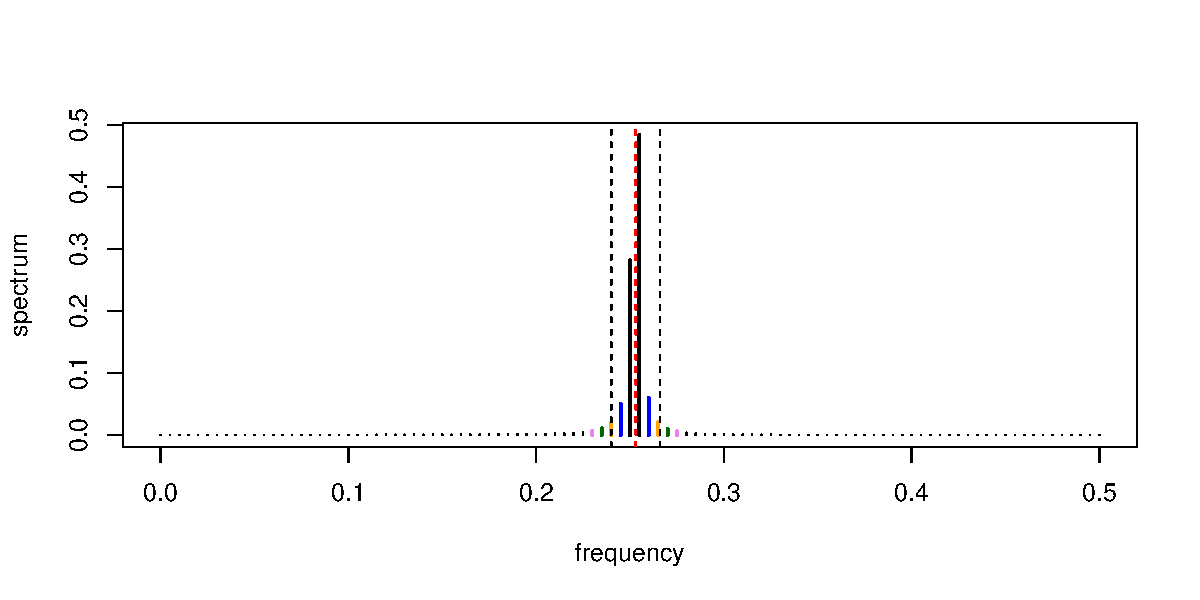
\includegraphics[width=\linewidth]{../img/Delta_example.pdf}
        \caption{$\Pi^{C, \omega}(k / N)$ и границы частотного интервала при $\delta=\delta^*$ ($N=200$, $C=2$, $\omega=0.253$, $\Sigma_t=0.9$, $\varepsilon=0.05$)}
        \label{fig:Delta_example}
    \end{figure}
    
\end{frame}

\begin{frame}{Метод autoMCSSA: преимущества и недостатки}
    
    \begin{itemize}
        \item \bluetext{Основное преимущество}: Метод позволяет выделять сигнал, компоненты которого в SSA разложении не обязательно доминируют.\medskip
        \item \textcolor{red}{Недостаток}: Если компоненты в SSA разложении неразделимы (это так, например, в случае гармоник с одинаковыми амплитудами), то описанный способ автоматической группировки перестает работать.\medskip
        \item \bluetext{Идея}: использовать метод после метода SSA-Aid, чтобы выделить компоненты, которые смешались с шумом.
    \end{itemize}

\end{frame}

\begin{frame}{Модификация отбора гармоник в методе SSA-Aid}

    Вместо последовательного выделения гармоник с наибольшей суммой квадратов, можно подойти более умно, используя преимущество MC-SSA перед другими критериями проверки ряда на наличие сигнала: информацию о значимой частоте. 

    \begin{algorithm}[Модификация отбора гармоник в методе SSA-Aid]
        \bluetext{Входные данные}: сгруппированные методом регулярности углов гармоники $\{\tX^{(j)}\}_{j\in J_{\text{Periodics}}}$, оценка максимально значимой частоты $\omega^\star$, порог $T_0$, верхняя граница величины амплитудной модуляции $C_\text{max}$.\medskip

        \bluetext{Результат}: множество $J_{\omega^\star}$ индексов, соответствующей частоте $\omega^\star$, оценка периодики $\tP_{\omega^\star}$.\medskip

        \begin{enumerate}
            \item Вычислить радиус $\delta_{\omega^\star}^*=\delta^*(\omega^\star, C_{\text{max}})$.\smallskip
            \item Получить множество $J_{\omega^\star}$ и оценку периодики $\tP_{\omega^\star}$ с помощью алгоритма автоматической идентификации гармоник с рядами $\left\{\tX^{(j)}\right\}_{j\in J_{\text{Periodics}}}$, $\delta=\delta_{\omega^\star}$ и $d=1$.
        \end{enumerate}
    \end{algorithm}

    % \begin{itemize}
    %     \item Основная идея: Использовать SSA-Aid для 
    %     \item Вместо последовательного выбора периодик с наибольшей суммой квадратов, модификация использует оценку значимой частоты (полученной с помощью MC-SSA) и идентифицирует периодику с помощью метода автоматической идентификации периодики.
    %     \item 
    % \end{itemize}
\end{frame}

\begin{frame}{Метод SSA-AidMC}

    \begin{figure}[H]
        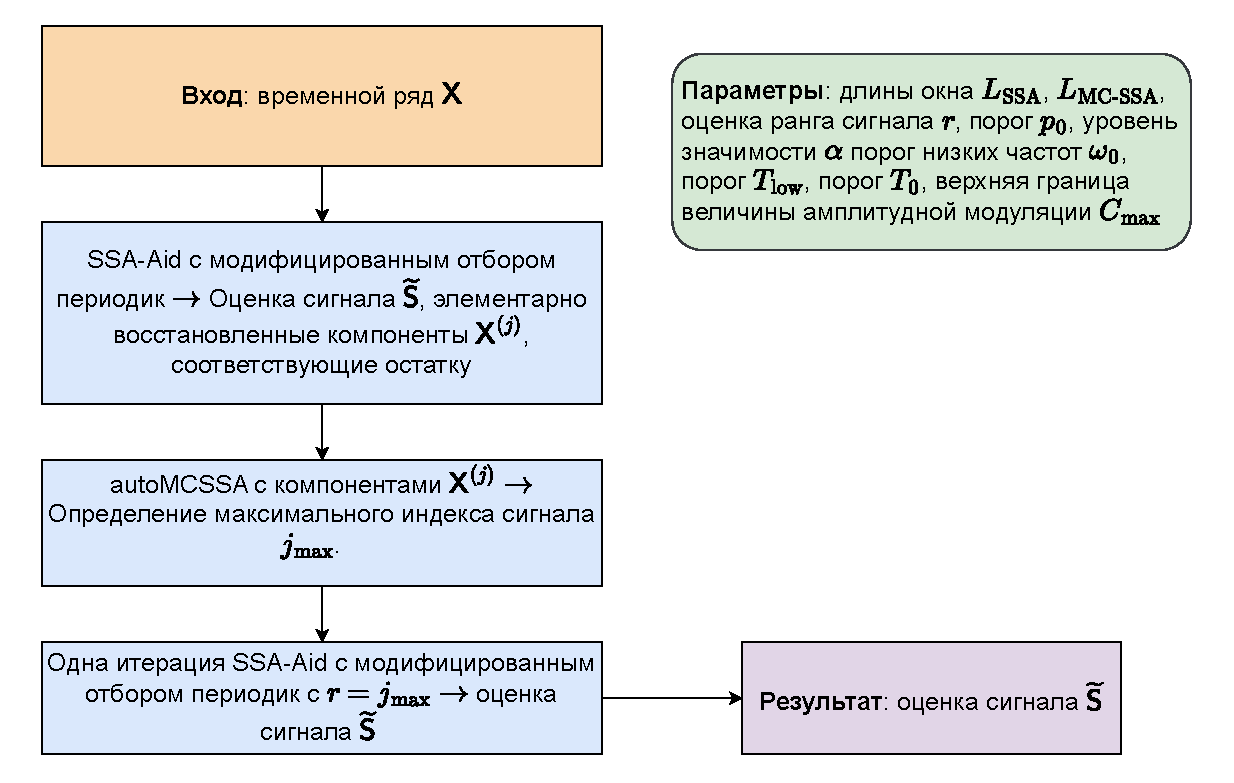
\includegraphics[width=0.98\linewidth]{../img/ssa_aidmc.pdf}
        \caption{Схема алгоритма SSA-AidMC}
    \end{figure}

\end{frame}

\begin{frame}{Численное сравнение точности идентификации компонент}

    \bluetext{Модель}: $\tX=\tT+\tP+\bm\xi$, где $N=200$, $\tT=(t_1,\ldots,t_N)$~--- тренд, $\tP=(p_1,\ldots,p_N)$, $\bm\xi$~--- красный шум с параметрами $\phi$ и $\sigma^2$.\medskip

    \bluetext{Задача}: сравнить методы autoMCSSA, SSA-Aid и SSA-AidMC по точности выделения различных сигналов.

    \begin{remark}
        Метод autoMCSSA умеет работать только с периодичностью. Однако можно сначала применить алгоритм autoEOSSA~[Golyandina, Dudnik, Shlemov and 2023] для выделения тренда, а потом применять autoMCSSA к остатку и с нетрендовыми элементарными компонентами.
    \end{remark}

\end{frame}

\begin{frame}{Численное сравнение точности идентификации компонент: сигнал доминирует над шумом}
    Рассмотрим примеры сигналов, доминирующих над шумом. Для таких сигналов выбраны следующие параметры алгоритмов:\smallskip
    \begin{enumerate}
        \item Длины окна $L_\text{SSA}=96$ и $L_\text{MC-SSA}=48$;\smallskip
        \item Порог низких частот $\omega_0=1/24$;\smallskip
        \item Пороги $T_\text{low}=T_0=0.5$;\smallskip
        \item Максимально возможная модуляция $C_{\max}=5$;\smallskip
        \item Оценка ранга сигнала $r=30$.\smallskip
    \end{enumerate}
    Также рассмотрим два случая параметра $\phi$: $\phi=0$ (белый шум) и $\phi=0.3$. Дисперсия белого шума $\sigma^2=1$ в обоих случаях.

\end{frame}

\begin{frame}{Численное сравнение точности идентификации компонент: сигнал доминирует над шумом}

    Пример 1:
    \begin{align*}
        t_n & =0.2 e^{0.025n} + 2\cos\left(\frac{2\pi n}{60}\right),                                            \\
        p_n & =4.12\cos\left(\frac{2\pi n}{4}\right) + 4.12\cos\left(\frac{2\pi n}{3}\right) + 6\cdot (-1)^{n}.
    \end{align*}

    \begin{table}[h!]
        \centering
        \caption{MSE восстановления сигнала, пример 1}
        \subfloat[Белый шум ($\sigma^2=1$)]{
            \scalebox{0.55}{\begin{tabular}{c|c|c|c}
                    Метод     & Компонента & Mean MSE & Median MSE \\
                    \hline
                    SSA-AidMC & Тренд      & 0.04372  & 0.03652    \\
                    \cline{2-4}
                              & Периодика  & 0.07700  & 0.06915    \\
                    \cline{2-4}
                              & Сигнал     & 0.12059  & 0.11141    \\
                    \hline
                    autoMCSSA & Тренд      & 0.063695 & 0.056327   \\
                    \cline{2-4}
                              & Периодика  & 0.15735  & 0.07171    \\
                    \cline{2-4}
                              & Сигнал     & 0.22069  & 0.14024    \\
                    \hline
                    SSA-Aid   & Тренд      & 0.04361  & 0.03652    \\
                    \cline{2-4}
                              & Периодика  & 0.07146  & 0.06594    \\
                    \cline{2-4}
                              & Сигнал     & 0.11494  & 0.10880    \\
                    \hline
                \end{tabular}}
        }\quad
        \subfloat[Красный шум ($\phi=0.3$, $\sigma^2=1$)]{
            \scalebox{0.55}{\begin{tabular}{c|c|c|c}
                    Метод     & Компонента & Mean MSE & Median MSE \\
                    \hline
                    SSA-AidMC & Тренд      & 0.10714  & 0.09391    \\
                    \cline{2-4}
                              & Периодика  & 0.05788  & 0.04978    \\
                    \cline{2-4}
                              & Сигнал     & 0.16477  & 0.15293    \\
                    \hline
                    autoMCSSA & Тренд      & 0.17468  & 0.15858    \\
                    \cline{2-4}
                              & Периодика  & 0.18239  & 0.05296    \\
                    \cline{2-4}
                              & Сигнал     & 0.35553  & 0.22301    \\
                    \hline
                    SSA-Aid   & Тренд      & 0.10617  & 0.09265    \\
                    \cline{2-4}
                              & Периодика  & 0.05377  & 0.04891    \\
                    \cline{2-4}
                              & Сигнал     & 0.15968  & 0.14524    \\
                    \hline
                \end{tabular}}
        }
    \end{table}

\end{frame}

\begin{frame}{Численное сравнение точности идентификации компонент: сигнал доминирует над шумом}

    Пример 2:
    \begin{align*}
        t_n & =0.2 e^{0.025n} + 2\cos\left(\frac{2\pi n}{60}\right),                                                           \\
        p_n & =4 e^{-0.01n}\cos\left(\frac{2\pi n}{4}\right) + 4\cos\left(\frac{2\pi n}{3}\right) + 6e^{-0.01n}\cdot (-1)^{n}.
    \end{align*}

    \begin{table}
        \centering
        \caption{MSE восстановления сигнала, пример 2}
        \subfloat[Белый шум ($\phi=0$, $\sigma^2=1$)]{
            \scalebox{0.55}{\begin{tabular}{c|c|c|c}
                    Метод     & Компонента & Mean MSE & Median MSE \\
                    \hline
                    SSA-AidMC & Тренд      & 0.04372  & 0.03652    \\
                    \cline{2-4}
                              & Периодика  & 0.07700  & 0.06915    \\
                    \cline{2-4}
                              & Сигнал     & 0.12059  & 0.11141    \\
                    \hline
                    autoMCSSA & Тренд      & 0.066280 & 0.053641   \\
                    \cline{2-4}
                              & Периодика  & 0.08458  & 0.07197    \\
                    \cline{2-4}
                              & Сигнал     & 0.1346   & 0.1261     \\
                    \hline
                    SSA-Aid   & Тренд      & 0.043611 & 0.036592   \\
                    \cline{2-4}
                              & Периодика  & 0.07146  & 0.06705    \\
                    \cline{2-4}
                              & Сигнал     & 0.1150   & 0.1087     \\
                    \hline
                \end{tabular}}
        }\quad
        \subfloat[Красный шум ($\phi=0.3$, $\sigma^2=1$)]{
            \scalebox{0.55}{\begin{tabular}{c|c|c|c}
                    Метод     & Компонента & Mean MSE & Median MSE \\
                    \hline
                    SSA-AidMC & Тренд      & 0.10714  & 0.09391    \\
                    \cline{2-4}
                              & Периодика  & 0.05788  & 0.04978    \\
                    \cline{2-4}
                              & Сигнал     & 0.16477  & 0.15293    \\
                    \hline
                    autoMCSSA & Тренд      & 0.14453  & 0.12942    \\
                    \cline{2-4}
                              & Периодика  & 0.06520  & 0.05408    \\
                    \cline{2-4}
                              & Сигнал     & 0.19250  & 0.18189    \\
                    \hline
                    SSA-Aid   & Тренд      & 0.10608  & 0.09286    \\
                    \cline{2-4}
                              & Периодика  & 0.05360  & 0.05103    \\
                    \cline{2-4}
                              & Сигнал     & 0.15936  & 0.14650    \\
                    \hline
                \end{tabular}}
        }
    \end{table}

\end{frame}

\begin{frame}{Численное сравнение точности идентификации компонент: шум доминирует над некоторыми компонентами сигнала}

    Рассмотрим примеры сигналов, некоторые компоненты которых не доминируют над шумом. Для таких сигналов выбраны следующие параметры алгоритмов:\smallskip
    \begin{enumerate}
        \item Длины окна $L_\text{SSA}=96$ и $L_\text{MC-SSA}=48$;\smallskip
        \item Порог низких частот $\omega_0=1/24$;\smallskip
        \item Пороги $T_\text{low}=T_0=0.5$;\smallskip
        \item Максимально возможная модуляция $C_{\max}=5$;\smallskip
        \item Оценка ранга сигнала $r=30$;\smallskip
        \item Поскольку шум будет достаточно сильным, порог для алгоритма SSA-Aid $t_0=0.5$, а для алгоритма SSA-AidMC $t_0=+\infty$ (то есть его нет).\smallskip
    \end{enumerate}
    Будем рассматривать красный шум с параметрами $\phi=0.7$ и $\sigma^2=1$.
    
\end{frame}

\begin{frame}{Численное сравнение точности идентификации компонент: шум доминирует над некоторыми компонентами сигнала}

    Пример 3:
    \begin{align*}
		p_n & =0.075 e^{0.02n}\cos\left(\frac{2 \pi n}{8}\right) + \cos\left(\frac{2 \pi n}{4}\right) + 0.2\cdot (-1)^n.
	\end{align*}

	\begin{table}
		\centering
        \caption{MSE восстановления сигнала, пример 3 ($\phi=0.7$, $\sigma^2=1$)}
		\begin{tabular}{c|c|c}
			Метод     & Mean MSE & Median MSE \\
			\hline
			SSA-AidMC & 0.10954  & 0.08997    \\
			\hline
			autoMCSSA & 0.15317  & 0.11806    \\
			\hline
			SSA-Aid   & 0.62960  & 0.53496    \\
			\hline
		\end{tabular}
	\end{table}
    
\end{frame}

\begin{frame}{Численное сравнение точности идентификации компонент: шум доминирует над некоторыми компонентами сигнала}

    Пример 4:
    \begin{align*}
		p_n =0.075 e^{0.02n}\cos\left(\frac{2 \pi n}{8}\right) &+ 1.5e^{-0.01n}\cos\left(\frac{2 \pi n}{4}\right)\\
        &+e^{-0.01n}\cdot (-1)^n.
	\end{align*}

	\begin{table}
		\centering
        \caption{MSE восстановления сигнала, пример 4 ($\phi=0.7$, $\sigma^2=1$)}
		\begin{tabular}{c|c|c}
			Метод     & Mean MSE & Median MSE \\
			\hline
			SSA-AidMC & 0.11023  & 0.09082    \\
			\hline
			autoMCSSA & 0.14604  & 0.11728    \\
			\hline
			SSA-Aid   & 0.84790  & 0.75026    \\
			\hline
		\end{tabular}
	\end{table}
    
\end{frame}

\begin{frame}{Численное сравнение точности идентификации компонент: выводы}

    Можно сделать следующие выводы:
    \begin{itemize}
        \item В случае доминирующего над шумом сигнала метод SSA-AidMC немного хуже метода SSA-Aid.\medskip
        \item В случае же сигналов, у которых некоторые компоненты не доминируют над шумом, SSA-AidMC является безоговорочным лидером. По ошибке восстановления сигнала метода SSA-Aid можно прийти к выводу, что он в данном случае неприменим.\medskip
        \item autoMCSSA показывает в обоих случаях результат хуже, чем SSA-AidMC в виду проблемы неразделимости компонент.
    \end{itemize}
    
\end{frame}

\begin{frame}{Заключение}
    \small
    Мои результаты:
    \begin{enumerate}
        \item Метод MC-SSA был обобщен на временные ряды с длинной памятью.
        \item Были разработаны и реализованы методы autoMCSSA и SSA-AidMC автоматической идентификации компонент, использующие критерий MC-SSA для определения значимых частот.
        \item На основании численных экспериментов были сделаны следующие выводы:
        \begin{itemize}\small
            \item Для оценки параметров шума предпочтительнее использовать метод Уиттла ввиду его меньшей трудоемкости и меньшего смещения оценок при неизвестном среднем.
            \item Критерий MC-SSA с косинусами в качестве проекционных векторов предпочтительнее критерия с векторами, порожденными исходным рядом. Такой выбор векторов избавляет от проблемы радикальности критерия с сохранением мощности.
            \item Метод SSA-AidMC показал себя намного лучше метода SSA-Aid в случае, когда сигнал не обязательно доминирует над шумом. С случае же, когда он доминирует, точность идентификации становится не сильно хуже.
        \end{itemize}
    \end{enumerate}
    
\end{frame}

\begin{frame}{Дальнейшие планы}
    
    \begin{enumerate}
        \item Добавить больше примеров рядов с длинной памятью.\medskip
        \item Провести больше сравнений SSA-AidMC с другими алгоритмами, в том числе на реальных данных.
    \end{enumerate}
    
\end{frame}

\end{document}